\documentclass{cheatsheet}
\begin{document}
	\setlist[itemize]{left=0pt}
	\title{高二 Cheatsheet}
	\rowcolors{2}{white}{blue!10}
	\renewcommand{\arraystretch}{1.5}
	\begin{tabularx}{\columnwidth}{XX}
		\rowcolor{blue!30}
		\multicolumn{2}{l}{\parbox[c][2.5\ht\strutbox][c]{0.9\columnwidth}{\Large 静电场（防止大家忘记）}} \\
		场强定义&$E=\frac Fq$\\
		电势定义&$\varphi = \frac Wq$\\
		电势差定义&$U_{AB}=\varphi_A-\varphi_B$\\
		电场力做功&$W=qU_{AB}=W_A-W_B=\varSigma qE\Delta d$\\
		\multicolumn{2}{l}{\textbf{匀强电场规律}}\\
		电势差与场强关系&$U=Ed$\\
		\multicolumn{2}{l}{\textbf{点电荷}}\\
		库仑定律&$F=\frac{kQq}{r^2}$\\
		点电荷电场强度&$E=\frac{kQ}{r^2}$\\
		点电荷电势&$\varphi=\frac{kQ}{r}$\\
	\end{tabularx}
	\notice{
		\begin{itemize}
			\item 电势能增加，一般情况下，机械能减少
			\item 判断电势能的增减，可以通过电场力做功，电场力做正功，电势能减小。
			\item 可以通过沿电场线方向电势降低，通过电荷正负与电势的计算式。
			\item 电场力做功注意需要进行投影，也就是$W=qEd\cos\theta$
			\item 电场线与等势面垂直
			\item 在匀强电场中，两点所在直线的场强均匀，可以通过$E^{'}=\frac Ud$求出。
		\end{itemize}
	}
	\notice{
		{
			游标卡尺读数方法：\\
			\centering
			
\includegraphics[width=\columnwidth]{assets/游标卡尺读数.jpg}
		}
		有两种方法读游标卡尺读数，\\
		\textbf{方法一}：下方副尺0刻度线所在位置主尺的读数记为$N$（上图应该是3cm处，但是不到31mm）\\
		然后找到副尺上与主尺刻度线对齐的刻度线的小格数，记为$m$，\\
		游标卡尺读数$=N+m\times \text{游标卡尺精度}$mm\\
		如上，为$ 30+6\times 0.1 \text{mm} = 30.6\text{mm}$\\
		\textbf{方法二}：找到主尺与副尺刻度线\textbf{对齐}所在位置的读数，记为$N$，\\
		找到副尺上与主尺刻度线\textbf{对齐}的刻度线对应的小格数，记为$m$，\\
		游标卡尺读数为$=N-\frac{\text{副尺总长度}}{\text{副尺总格子数}}\times m$mm\\
		如上，为$ 36 - \frac{6}{10}\times 9 \text{mm} = 30.6\text{mm}$\\
	}
	\notice{
		{
			螺旋测微器读数方法：\\
			\centering
			
\includegraphics[width=\columnwidth]{assets/螺旋测微器读数.jpg}
		}
		先确定右侧旋转筒左侧线所指的主尺半格数，注意上面也有一排刻度线，当超过主尺刻度线时，主尺读数需要加0.5mm，\\
		然后读取右侧旋转筒上与主尺左侧线对齐的刻度线数，乘以螺旋测微器的精度0.01mm，注意需要估读一位，尽量估读准确一点。\\
		最后螺旋测微器读数$=$主尺读数$+$旋转筒读数。\\
		如上，为$ 6.5 \text{mm} + 20.3\times 0.01 \text{mm} = 6.703\text{mm}$\\
	}
	\begin{tabularx}{\columnwidth}{XX}
		\rowcolor{blue!30}
		\multicolumn{2}{l}{\parbox[c][2.5\ht\strutbox][c]{0.9\columnwidth}{\Large 电路基本元件}} \\
		电流定义式&$I=\frac Qt$\\
		电流决定式&$I = nqSv$\\
		电阻定义式&$R=\frac UI$\\
		电阻决定式&$R=\rho\frac lS$\\
		电容定义式&$C=\frac QU$\\
		电容决定式&$C=\frac{\epsilon S}{4\pi kd}$\\
		电源电动势&$E=\frac{W_{\text{非静电力}}}{q}$\\
	\end{tabularx}
	\begin{tabularx}{\columnwidth}{XX}
		\rowcolor{blue!30}
		\multicolumn{2}{l}{\parbox[c][2.5\ht\strutbox][c]{0.9\columnwidth}{\Large 闭合电路欧姆定律}} \\
		不含外电路电压&$E=I(R+r)$\\
		不含内阻和电动势&$U=IR$\\
		不含外电阻&$U=E-Ir$\\
		不含电流&$U=E\frac{R}{R+r}$\\
		串联规律&$R=R_1+R_2+\cdots R_n$\\
		并联规律&$\frac1R=\frac1{R_1}+\frac1R_2+\cdots \frac1R_n$\\
	\end{tabularx}
	\notice{
		\begin{itemize}
			\item 恒压源的正极电势恒定比负极大$E$。
			\item 恒流源干路电流恒定为$I$。（实际上两种电源就是按照上面的原则列欧姆定律方程）
			\item 沿电流方向电势降低
			\item 电势降低量$U=RI$
			\item 对电路中任意节点：$\Sigma I_{in}=\Sigma I_{out}$（如果定义的电流没有流出或者没有流入，那么认为是0。）
			\item 导线的内阻为0，所以导线可以任意长度变化，注意测电阻率时，电阻丝不认为是导线，而是纯电阻。
			\item 理想电流表视为导线，理想电压表视为断路。
			\item 电容器充满电或者稳定状态都视为断路，
			\item 电容器充电过程视为电阻，
			\item 电容器放电视为理想电源。
			\item 断路应该被视为是一个无穷大的电阻接在断路的导线两端。
			\item 任何部分电阻增大都会导致总电阻增大，反之亦然。（该方法可以快速判断总电阻）
		\end{itemize}
	}
	\begin{tabularx}{\columnwidth}{XX}
		\rowcolor{blue!30}
		\multicolumn{2}{l}{\parbox[c][2.5\ht\strutbox][c]{0.9\columnwidth}{\Large 电表改装}} \\
		电流表简易改装&$R=\frac{I_gR_g}{I_{\text{量程}}-I_g}\approx \frac{I_gR_g}{I_{\text{量程}}}$\\
		电压表简易改装&$R=\frac{U_{\text{量程}}}{I_g}-R_g$\\
		欧姆表改装&$E=i(r+R_g+R_{\Omega}+R_x)$\\
		欧姆表量程刻度&$R_x=\frac{E}{i}-\frac{E}{I_g}=E\frac{I_g-i}{iIg}$\\
		&$R_x=R_{\text{内}}(\frac{I_g}{i}-1)$\\
		欧姆表中值电阻&$R_{\text{中值电阻}}=\frac{E}{I_g}=R_{\text{内}}$\\
	\end{tabularx}
	\hint{
		多用电表使用，首先进行机械调零，旋转机械调零螺丝让指针指到电流表的0刻度线。注意这个名字，机械调零螺丝，欧姆调零旋钮。\\
		\\
		如果使用欧姆表测电阻，\\
		1. 首先选择合适挡位\\
		2. 进行欧姆调零，红黑表笔短接，\\
		3. 旋转欧姆调零旋钮让指针指到电流表满偏位置（同时也是欧姆表0刻度线）。\\
		每次换挡都需要进行欧姆调零。\\
		\\
		关于红黑表笔问题，多用电表与电流表电压表都是符合“红进黑出”原则的，\\
		对于电流表和电压表，电流来自外部电路，所以红表笔与电流流出节点相连，
		比如电源的电流从正极流出，所以\\
		\colorbox{yellow}{\textit{电流表红色端与电源正极相连}}。\\
		对于欧姆表，电流来自欧姆表内部电源，所以\colorbox{yellow}{\textit{黑表笔与内部电源的正极相连}}，这样电流就会从黑表笔流出经过外部电阻，红表笔就和内部电源的负极相连，电流同样流入。
	}
	\hint{
		上面的改装原理可以解释为什么电流表和电压表表盘是均匀的，而欧姆表的表盘不均匀。\\
		通过电流表改装的公式可以得到：
		\[\frac{i}{I}=\frac{R}{R+R_g}\]
		\[\frac{i_{\text{表头电流}}}{I_{\text{干路电流}}}=\frac{I_g}{I_{\text{满偏}}}\]
		即，改装后的电流表，表头电流与干路电流成正比，那么可以利用表头读数计算干路电流，并且是线性的关系。\\
		
		
		通过电压表改装的公式可以得到：
		\[i=\frac{U_\text{总}}{R+R_g}\]
		即总电压与表头电流成正比，那么可以利用表头读数计算总电压，并且是线性的关系。\\
		
		
		通过欧姆表改装的公式可以得到：
		\[i=\frac{E}{R_{\text{内}}+R_x}\]
		即，表头电流与被测电阻成反比，表盘才会不均匀，并且电阻越大，电流变化幅度越小，左边的刻度偏角间隔就会越小。\\
	}
	\begin{tabularx}{\columnwidth}{XX}
		\rowcolor{blue!30}
		\multicolumn{2}{l}{\parbox[c][2.5\ht\strutbox][c]{0.9\columnwidth}{\Large 用电器功率和电源功率}} \\
		电功率定义式&$P=UI$\\
		\multicolumn{2}{l}{\textbf{用电器功率}}\\
		纯电阻功率&$P=P_{\text{热}}=I^2R=\frac{U^2}{R}$\\
		非纯电阻总功率&$P=UI$\\
		非纯电阻热功率&$P=I^2R$\\
		非纯电阻输出功率&$P=UI-I^2R$\\
		\multicolumn{2}{l}{\textbf{电源功率}}\\
		电源总功率&$P=EI=\frac{E^2}{R+r}\le \frac{E^2}{r}$\\
		电源热功率&$P=I^2r=(\frac{E}{R+r})^2r\le \frac{E^2}{r}$\\
		电源输出功率&$P=UI=(E-Ir)I=(\frac{E}{r}-I)Ir\le \frac{E^2}{4r}$\\
		包含纯电阻电源输出功率&$P=(\frac{E}{R+r})^2R$\\
		电源效率&$\eta=\frac{P_{\text{输出}}}{P_{\text{总}}}=\frac U E=\frac{R}{R+r}$\\
	\end{tabularx}\\
	\notice{
		上面的小于等于的意思是，存在一个极大值。
	}
	\hint{
		\begin{itemize}
			\item 正常工作意味着用电器的全部物理量为额定值
			\item 电动机这样的非纯电阻元器件，不能正常工作，可以看作纯电阻。
			\item 灯泡虽然会发热，但是仍然看成定值电阻。
			\item \textbf{不要使用非纯电阻两端电压得到电流或者电阻。$r\neq \frac UI$}
			\item 非纯电阻的内阻也不要与其他电路电阻进行串并联。
		\end{itemize}
	}
	{
		\centering
		\textbf{电源功率与电流图像}\\
		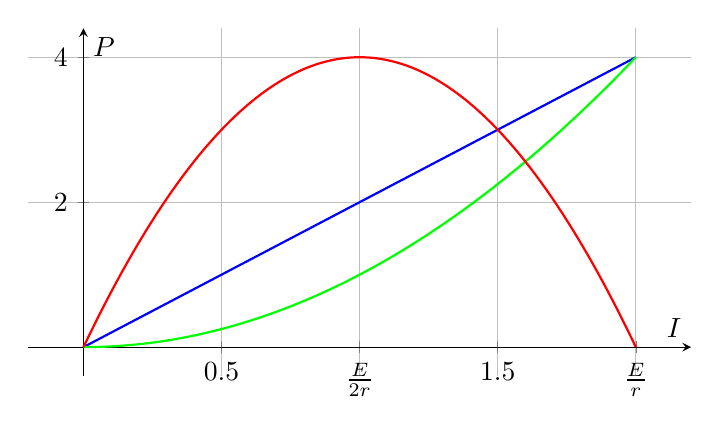
\begin{tikzpicture}
			\begin{axis}[
				width=10cm, height=6cm,
				axis lines=middle,
				xlabel={$I$},
				ylabel={$P$},
				xtick={0,0.5,1,1.5,2},
				xticklabels={0,0.5,$\frac {E}{2r}$,1.5,$\frac{E}{r}$},
				xmin=0, xmax=2,
				ymin=0, ymax=4,
				grid=both,
				samples=100,
				domain=0:2,
				enlargelimits
				]
				\addplot[blue, thick] {2*x}; % E = 4V 为示例
				\addplot[green, thick] {(x*x)*1)};
				\addplot[red, thick] {4*x*(2-x)};
			\end{axis}
		\end{tikzpicture}\\
		\textbf{电源功率与外电阻图像}\\
		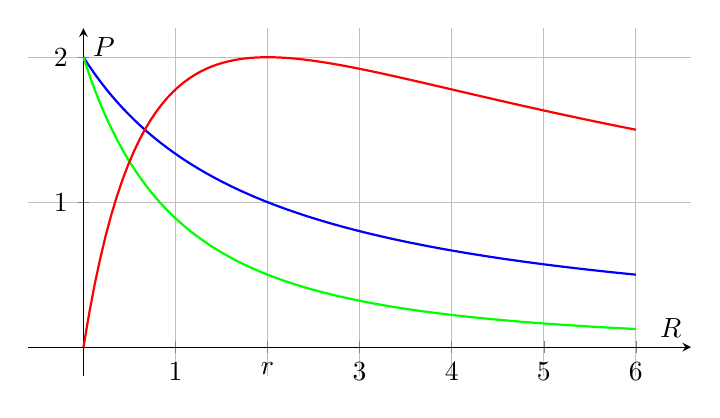
\begin{tikzpicture}
			\begin{axis}[
				width=10cm, height=6cm,
				axis lines=middle,
				xlabel={$R$},
				ylabel={$P$},
				xtick={0,1,2,3,4,5,6},
				xticklabels={0,1,$r$,3,4,5,6},
				xmin=0, xmax=6,
				ymin=0, ymax=2,
				grid=both,
				samples=100,
				domain=0:6,
				enlargelimits
				]
				\addplot[blue, thick] {4/(2+x)}; % E = 4V 为示例
				\addplot[green, thick] {8/((2+x)^2)};
				\addplot[red, thick] {16*x/((2+x)^2)};
			\end{axis}
		\end{tikzpicture}\\
		\textbf{电源功率与外电压图像}\\
		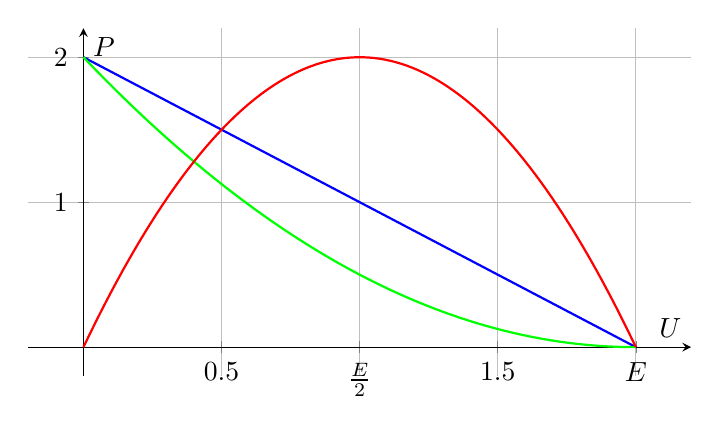
\begin{tikzpicture}
			\begin{axis}[
				width=10cm, height=6cm,
				axis lines=middle,
				xlabel={$U$},
				ylabel={$P$},
				xtick={0,0.5,1,1.5,2},
				xticklabels={0,0.5,$\frac E2$,1.5,$E$},
				xmin=0, xmax=2,
				ymin=0, ymax=2,
				grid=both,
				samples=100,
				domain=0:2,
				enlargelimits
				]
				\addplot[blue, thick] {2-x}; % E = 4V 为示例
				\addplot[green, thick] {0.5*(2-x)^2)};
				\addplot[red, thick] {2*x*(2-x)};
			\end{axis}
		\end{tikzpicture}\\
	}
	$\frac Er$为短路电流，\\
	蓝色直线为电源总功率，\\
	绿色抛物线为电源热功率，\\
	红色抛物线为电源输出功率，电阻线经过了4倍放大，这样能够清晰地看出输出功率随电阻变化先增大后减小，在内阻等于外阻的时候取得极值。\\
	\notice{
		通过输出功率最大时电阻情况，可以知道，此时内外电压相等，大小为$\frac E2$，\\
		外电阻增大，电源总功率和电源热功率都会减小，电源效率也会升高。\\
		增加的功率与外电压的图像中，可以发现，外电压增大，输出功率先增大后减小，\\
		当外电压等于$\frac E2$时，输出功率最大，此时电源效率为50\%。\\
		\textit{如果题目是外电阻固定，改变内阻请一定要结合欧姆定律进行分析，不要强行套结论。}
	}
	\hint{
		电流表内接时，因为电流表分压，电阻测量值偏大，\\
		电流表外接时，因为电压表分流，电阻测量值偏小。\\
		\\
		判断电表接法时，首先应当确认电表的内阻是否是准确值，\\
		如果是估算的内阻已知，那么请务必采用下面结论。\\
		电流表内阻已知，采用内接法；\\
		电流表内阻未知，采用外接法。\\
		\\
		除此之外采用下面的两种方法判断：\\
		临界值法，\\
		如果$R_x<\sqrt{R_VR_A}$，外接；\\
		如果$R_x>\sqrt{R_VR_A}$，内接。\\
		试触法，\\
		如果两次内外接过程中，\\
		电流表读数变化较大，即电压表分流明显，采用内接法；\\
		电压表读数变化较大，即电流表分压明显，采用外接法。\\
		\\
		电表量程选择时，可以略超量程，但是不能选择过大的量程，例如，电源电压为4V，选择3V的电压表是可行的。但是选择15V的电压表就不合适了。\\
	}
	
	{
		\centering
		\textbf{电流表外接法与滑动变阻器分压式接法}\\
		\begin{adjustbox}{scale=0.8,center}
			\begin{circuitikz}[european resistors]
				\tikzstyle{every node}=[font=\LARGE]
				\draw (7.5,16.5) to[battery] (10,16.5);
				\draw (7.5,17.75) to[potentiometer] (12.5,17.75);
				\draw (10,16.5) to[normal open switch] (12.5,16.5);
				\draw (10,18.25) to[short] (10,19);
				\draw (10,19) to[short] (12.5,19);
				\draw (12.5,16.5) to[short] (12.5,17.75);
				\draw (12.5,19) to[short] (12.5,21.5);
				\draw (7.5,21.5) to[rmeter, t=V] (12.5,21.5);
				\draw (7.5,20.25) to[european resistor] (12.5,20.25);
				\draw (7.5,16.5) to[rmeter, t=A] (7.5,21.5);
			\end{circuitikz}
		\end{adjustbox}
	}\newpage
	{
		\centering
		\textbf{电流表内接法与滑动变阻器限流式接法}\\
		\begin{adjustbox}{scale=0.8,center}
			\begin{circuitikz}[european resistors]
				\tikzstyle{every node}=[font=\LARGE]
				\draw (7.5,16.5) to[battery ] (10,16.5);
				\draw (10,16.5) to[normal open switch] (11.25,16.5);
				\draw (11.25,16.5) to[potentiometer] (13.75,16.5);
				\draw (7.5,17.75) to[european resistor] (10,17.75);
				\draw (10,17.75) to[rmeter, t=A] (12.5,17.75);
				\draw (7.5,19) to[rmeter, t=V] (12.5,19);
				\draw (7.5,16.5) to[short] (7.5,19);
				\draw (12.5,17) to[short] (12.5,17.75);
				\draw (12.5,17.75) to[short] (12.5,19);
			\end{circuitikz}
		\end{adjustbox}
	}\\
	\hint{
		滑动变阻器选取按照如下原则，依次进行。
		\begin{itemize}
			\item 要求大范围，电压或电流从0开始，测量用电器伏安特性曲线，分压式接法。
			\item 滑动变阻器总电阻小于用电器，分压式接法。
			\item 滑动变阻器总电阻和用电器接近，限流式接法。
			\item 需要节省能量，尽可能节约，限流式接法。
		\end{itemize}
	}

\end{document}
